\documentclass[9pt]{beamer}

%!TEX root = ../notas_de_clase.tex

%preamble

%language
\usepackage[spanish,es-nodecimaldot]{babel}
\usepackage[utf8]{inputenc}
\usepackage{apacite}
\usepackage[absolute,overlay]{textpos}

%packages
\usepackage[Algoritmo]{algorithm}
\usepackage{algorithmicx}
\usepackage[noend]{algpseudocode}
\usepackage{mathtools}
\setlength {\marginparwidth}{2cm}
\usepackage{todonotes}
\usepackage{amsbsy}
\usepackage{amssymb}
\usepackage{amsmath,bm}
\usepackage{dsfont}

\usepackage{xcolor}
\providecommand{\sred}[1]{\textcolor{red}{#1}}
\providecommand{\sblue}[1]{\textcolor{blue}{#1}}
\providecommand{\red}[1]{\textcolor{red}{\text{#1}}}
\providecommand{\blue}[1]{\textcolor{blue}{\text{#1}}}
\providecommand{\redb}[1]{\textcolor{red}{\textbf{#1}}}
\providecommand{\blueb}[1]{\textcolor{blue}{\textbf{#1}}}
\usepackage{graphicx}
\usepackage{fancybox}
\usepackage{booktabs}
\usepackage{caption}
\usepackage{float}
%\usepackage[longend,ruled,algochapter,linesnumbered,lined,boxed,commentsnumbered,spanish]{algorithm2e}
%\usepackage[algo2e]{algorithm2e}
\usepackage{amssymb}
\usepackage{amstext}
\usepackage{bm}
\usepackage{wrapfig}
\usepackage{subcaption} % para_unsupervised_chapter

%formatting

\usepackage[export]{adjustbox}

%caption para figuras
\captionsetup[figure]{width=.8\linewidth, font=small,labelfont={bf},name={Fig.},labelsep=period}
\captionsetup[table]{width=.8\linewidth,font=small,labelfont={bf},name={Tabla},labelsep=period}



\ifx\byn\undefined
    \definecolor{my_blue}{HTML}{C2D5FF}
    \definecolor{my_red}{HTML}{FFC2C2}
    \definecolor{my_yellow}{HTML}{FFFFE0}
\else
    \definecolor{my_blue}{HTML}{FFFFFF}
    \definecolor{my_red}{HTML}{FFFFFF}
    \definecolor{my_yellow}{HTML}{FFFFFF}
\fi


\usepackage[framemethod=TikZ]{mdframed}
\mdfdefinestyle{discusion}{%
    %linecolor=black,
    %outerlinewidth=0pt,
    roundcorner=0pt,
    innertopmargin=5pt,
    innerbottommargin=5pt,
    innerrightmargin=20pt,
    innerleftmargin=20pt,
    backgroundcolor=my_blue}

\colorlet{Green}{green!90}


\mdfdefinestyle{ejemplo}{%
    %linecolor=black,
    %outerlinewidth=0pt,
    roundcorner=0pt,
    innertopmargin=5pt,
    innerbottommargin=5pt,
    innerrightmargin=20pt,
    innerleftmargin=20pt,
    backgroundcolor=my_yellow}


\mdfdefinestyle{pendiente}{%
    style = discusion, 
    backgroundcolor=my_red}


\RequirePackage{url}



%definitions
\def\td{{\text d}}
\def\cN{{\mathcal N}}
\def\cX{{\mathcal X}} 
\def\cC{{\mathcal C}} 
\def\N{{\mathbb N}}
\def\d{{\text d}}
\def\datos{{\mathcal D}}
\def\eye{{\mathbb I}}
\def\ssum{{\scriptstyle\sum}}
\def\bepsilon{{\bm \epsilon}}
\def\tx{\tilde{x}}
\def\tX{\tilde{X}}
\def\thetaMAP{\theta_\text{MAP}}
\newcommand{\gp}{\ensuremath{\mathcal{GP}}}
\newcommand{\pr}{\ensuremath{\mathbb{P}}}
\newcommand{\x}{\ensuremath{\mathbf{x}}}
\newcommand{\z}{\ensuremath{\mathbf{z}}}
\newcommand{\cvector}{\ensuremath{\mathbf{c}}}
\newcommand{\e}{\ensuremath{\mathbf{e}}}
\newcommand{\y}{\ensuremath{\mathbf{y}}}
\newcommand{\bx}{\ensuremath{\textcolor{blue}{X}}}
\newcommand{\by}{\ensuremath{\textcolor{blue}{Y}}}
\newcommand{\rx}{\ensuremath{\textcolor{red}{X_*}}}

\newcommand{\R}{\mathbb{R}}
\newcommand{\norm}[1]{\left\lVert#1\right\rVert}




\DeclareMathOperator*{\argmax}{arg\,max}
\DeclareMathOperator*{\argmin}{arg\,min}
\DeclareMathOperator{\E}{\mathbb{E}}
\DeclareMathOperator{\V}{\mathbb{V}}
\DeclareMathOperator{\KL}{\text{KL}}
\DeclareMathOperator{\MVN}{\text{MVN}}
\newcommand\deq{\stackrel{\mathclap{\normalfont\mbox{\tiny def}}}{=}}
%\newcommand{\E}[1]{\mathbb E \left[#1\right]}
\newcommand{\trace}[1]{\text{Tr} \left[#1\right]}


\usepackage{amsthm}

%-------------------------------------------
% Newtheorem
%-------------------------------------------
\newtheorem{axioma}{\textcolor{red}{Axioma}}
\newtheorem{definicion}{Definición}
\newtheorem*{notacion}{Notación}
\newtheorem{teorema}{Teorema}
\newtheorem{corolario}{Corolario}
\newtheorem{lema}{Lema}
\newtheorem{lemaZ}{\textcolor{red}{Lema}}
\newtheorem{propiedad}{Propiedad:}
\newtheorem{proposicion}{Proposición:}
\newtheorem*{observacion}{Observación}
\newtheorem*{comentario}{Comentario}
\newtheorem*{ejemplo}{Ejemplo}
\newtheorem*{resultado}{Resultado}
\newtheorem*{propuesto}{Ejercicio propuesto}
\newtheorem*{demostracion}{Demostración} % No se usa, usar \begin{proof}\end{proof} que son por default.

%listing paackage para código
\usepackage{listings}
\usepackage{xcolor}
 
\definecolor{codegreen}{rgb}{0,0.6,0}
\definecolor{codegray}{rgb}{0.5,0.5,0.5}
\definecolor{codepurple}{rgb}{0.58,0,0.82}
\definecolor{backcolour}{rgb}{0.95,0.95,0.92}
 
\lstdefinestyle{mystyle}{
    xleftmargin=0.15\textwidth,
    linewidth=0.8\textwidth,
    backgroundcolor=\color{backcolour},   
    commentstyle=\color{codegreen},
    keywordstyle=\color{magenta},
    numberstyle=\tiny\color{codegray},
    stringstyle=\color{codepurple},
    basicstyle=\ttfamily\footnotesize,
    breakatwhitespace=true,         
    breaklines=true,                 
    captionpos=b,                    
    keepspaces=true,                 
    numbers=left,                    
    numbersep=5pt,                  
    showspaces=false,                
    showstringspaces=false,
    showtabs=false,                  
    tabsize=2
}
 
\lstset{style=mystyle}

\numberwithin{equation}{section}

\usetheme{simple}

\title{Clase 21 - Procesos Gaussianos II}
\subtitle{Aprendizaje de Máquinas - MA5204}
\date{\today}
\author{Felipe Tobar} 
\titlegraphic{
\begin{figure}[htp] 
    \centering
        
\includegraphics[width=0.15\textwidth]{../img/Uchile.pdf}% 
\end{figure}
}
\institute{Department of Mathematical Engineering \&\\ Center for Mathematical Modelling\\Universidad de Chile}

\begin{document}
\begin{frame}
  \titlepage
\end{frame}

\section{Procesos Gaussianos - Entrenamiento y Optimización} 

\begin{frame}{¿Qué es entrenar un $\gp$?}
    Vimos que dada una función de covarianza podemos representar el proceso, y podemos encontrar analíticamente la densidad posterior de nuestra función $f(\cdot)$ condicionando a las observaciones. Pero la forma que tendrá la posterior y la función fuera de las observaciones dependerá fuertemente en nuestra función kernel escogida, en este sentido, para un kernel dado nos gustaría encontrar los parámetros de este que mejor representen nuestra función a estimar.
    \vspace{0.2cm} \pause 

    Nos referiremos a entrenar u optimizar un $\gp$ cuando queremos obtener los hyperparámetros, es decir los parámetros del kernel (los denotamos $\theta$) y la varianza del ruido (la denotamos $\sigma_n^2$) si es que aplica.

    
\end{frame}

\begin{frame}{Procesos Gaussianos - Entrenamiento}

    Consideremos la \textit{verosimilitud marginal}, obtenida marginalizando sobre la función $f(\cdot)$, donde dado un conjunto de entrenamiento $(X, Y)= \{(x_i, y_i)\}_{i=1}^{n}$, esta dada por \pause

    \begin{align*}
        \pr(Y|X, \theta, \sigma) & = \int \pr(Y|f, X, \theta, \sigma_n) p(f|X,\theta, \sigma) df \\
        & = \frac{1}{\left( 2\pi |\mathbf{K}_y|\right)^{\frac{n}{2}}} 
        \exp \left(
        -\frac{1}{2} (Y - \mathbf{m})^T \mathbf{K}_y^{-1} (Y - \mathbf{m})
        \right)
    \end{align*} \pause 
    
    Donde $\mathbf{m}=m(X)$ y $\mathbf{K}_y=K_{\theta}(X,X) + \sigma_n^2 \eye$, la matriz de covarianza dados los parámetros $\theta$ agregando el término de la diagonal correspondiente al ruido.\\ \pause 
    Considerando la log-verosimilitud negativa (NLL)

    \begin{align*}
        NLL & = -\log \pr(Y|X, \theta, \sigma_n) \\
        NLL & = \underbrace{ \color{black}{\frac{1}{2}\log|\mathbf{K_y}|} }_
            {\text{\parbox{2cm}{\centering Penalización\\[-4pt] por\\[-4pt] complejidad}}}
            + \underbrace{ \color{black}{\frac{1}{2}(Y - \mathbf{m})^T \mathbf{K}_y^{-1} (Y - \mathbf{m}) }}_
            {\text{\parbox{4cm}{\centering Data fit (Única parte que depende de $Y$)}}}
            + \underbrace{ \color{black}{\frac{n}{2} \log2\pi}}_
            {\text{\parbox{2cm}{\centering Constante de normalización}}}
    \end{align*}

    
\end{frame}

\begin{frame}{Procesos Gaussianos - Entrenamiento}
    \begin{figure}[H]
        \centering
        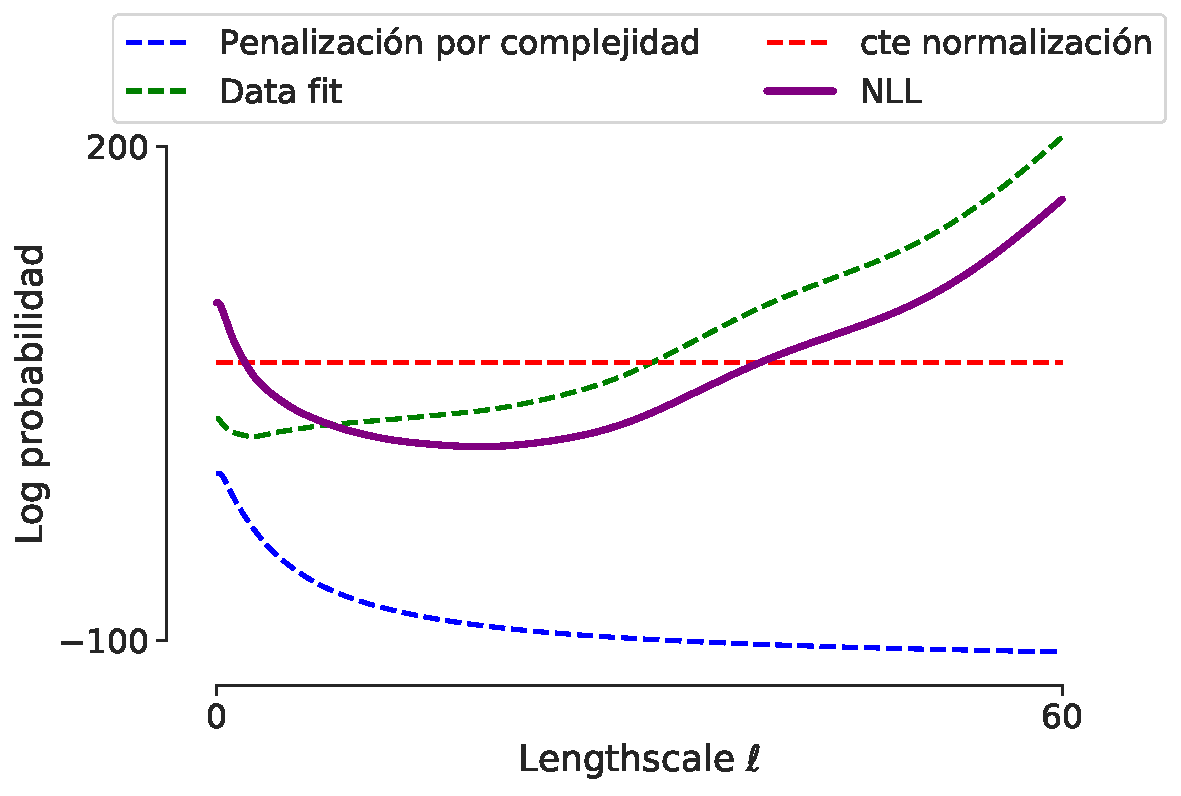
\includegraphics[width=0.7\textwidth]{../img/cap8_nll_partes}
        \caption{Log verosimilitud marginal negativa (NLL) en función del \textit{lengthscale} ($\ell$) para señal sintetica, se mantienen constantes los otros parámetros del $\gp$.}
    \end{figure}
\end{frame}

\begin{frame}{Procesos Gaussianos - Optimización}
Como contamos con una expresión cerrada para la NLL, podemos utilizar métodos clásicos de optimización, utilizando L-BFGS en el ejemplo anterior \pause 

    \begin{table}[H]
        \centering
        \begin{tabular}{lcccc}
         & $\sigma_{\text{ruido}}$ & $\ell$ & $\sigma_{\text{señal}}$ & NLL\\ \hline
        Sin entrenar & 0.2 & 3.1622 & 1 & $\mathbf{55.3538}$\\
        Entrenado & 0.2067 & 18.7267 & 0.9956 & $\mathbf{17.6945}$\\
        \end{tabular}
    \end{table} \pause 
        
        
    \begin{figure}[H]
            \centering
            \visible<3->{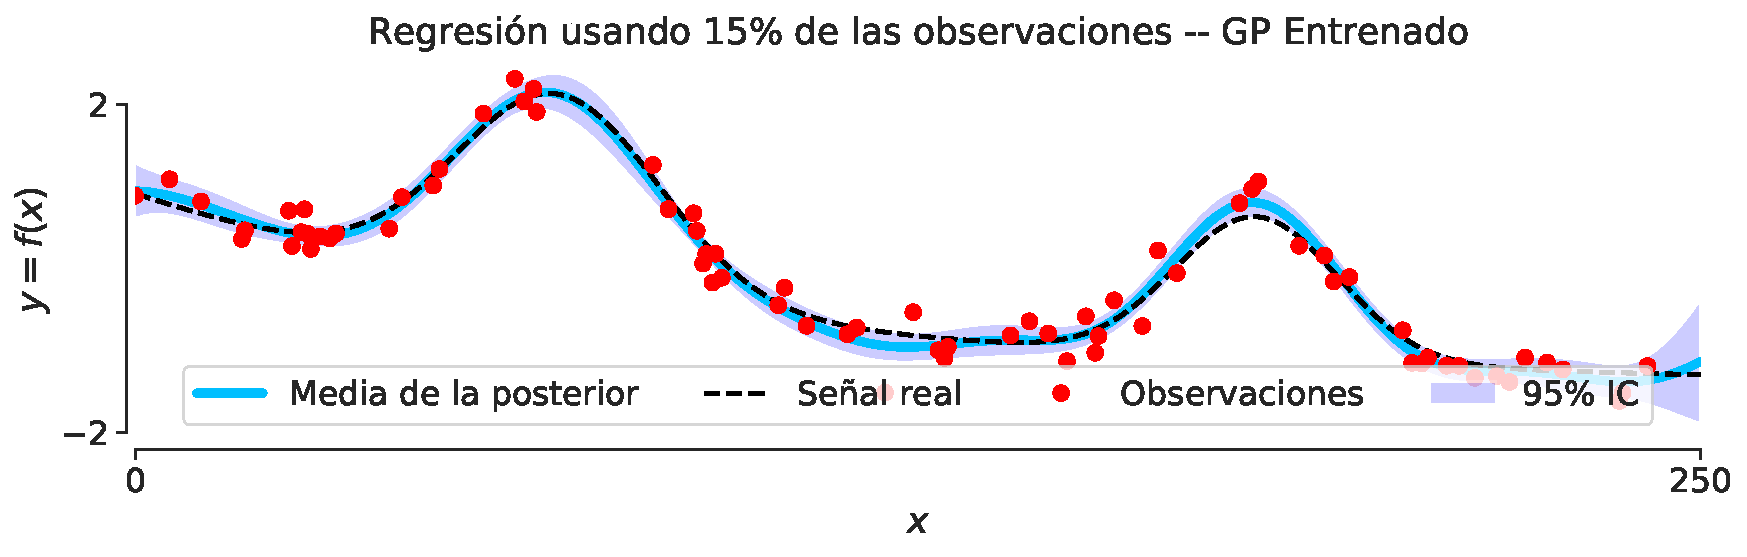
\includegraphics[width=0.9\textwidth]{../img/cap8_entrenado}}
            \caption{Regresión con $\gp$ para señal sintetica usando el 15$\%$ de los datos muestreados de forma no uniforme y contaminados con ruido Gaussiano, utilizando un $\gp$ de media nula y kernel SE; Modelo optimizado utilizando L-BFGS.}
    \end{figure}
\end{frame}


\begin{frame}{Función de covarianza (kernels)}
    Hasta el momento solo hemos utilizado un tipo de función de covarianza, el llamado kernel \textit{Squared Exponential} (SE), conocido también como kernel RBF. En esta sección mostraremos distintos tipos de funciones de covarianza y los distintos tipos de funciones que generan. \pause 

    \begin{equation*}
	K_{SE}(x, x') = \sigma^2 \exp\left( - \frac{\left( x- x'\right)^2}{2\ell^2} \right)
    \end{equation*} \pause 

    Es importante denotar tipos de familias de funciones de covarianza, si la función solo depende de la diferencia, es decir $k(x, x')=k(x-x')$ se le llamará \textit{kernel estacionario}, más aún, si depende solo de la norma de la diferencia $k(x, x')=k(|x-x'|)$ se le llamará \textit{kernel isométrico}, un ejemplo de esto es el kernel SE. \pause \vspace{0.2cm}

    Es de notar que kernels estacionarios hacen que la covarianza entre puntos sea invariante a traslaciones en el espacio de entradas. Una noción importante es que un kernel puede ser visto como una medida de similaridad entre puntos, y en el caso de kernels estacionarios, mientras más cercanos estén dos puntos más símiles serán. \\

    A continuación se presentan algunos tipos de kernel:
    
\end{frame}

\begin{frame}{Rational Quadratic (RQ)}


    Este kernel viene dado por la siguiente expresión 
 
    \begin{equation*}\label{eq:gp_kernel_rq}
	K_{RQ}(x, x') = \sigma^2 \left(1 + \frac{\left( x- x'\right)^2}{2\alpha\ell^2 } \right)^{-\alpha}
    \end{equation*}

    donde $\alpha$ es un parámetro de variación de escala, notar que cuando $\alpha \rightarrow \infty$ el kernel tiende a uno SE. \pause

    \begin{figure}[H]
	    \centering
	    \visible<2->{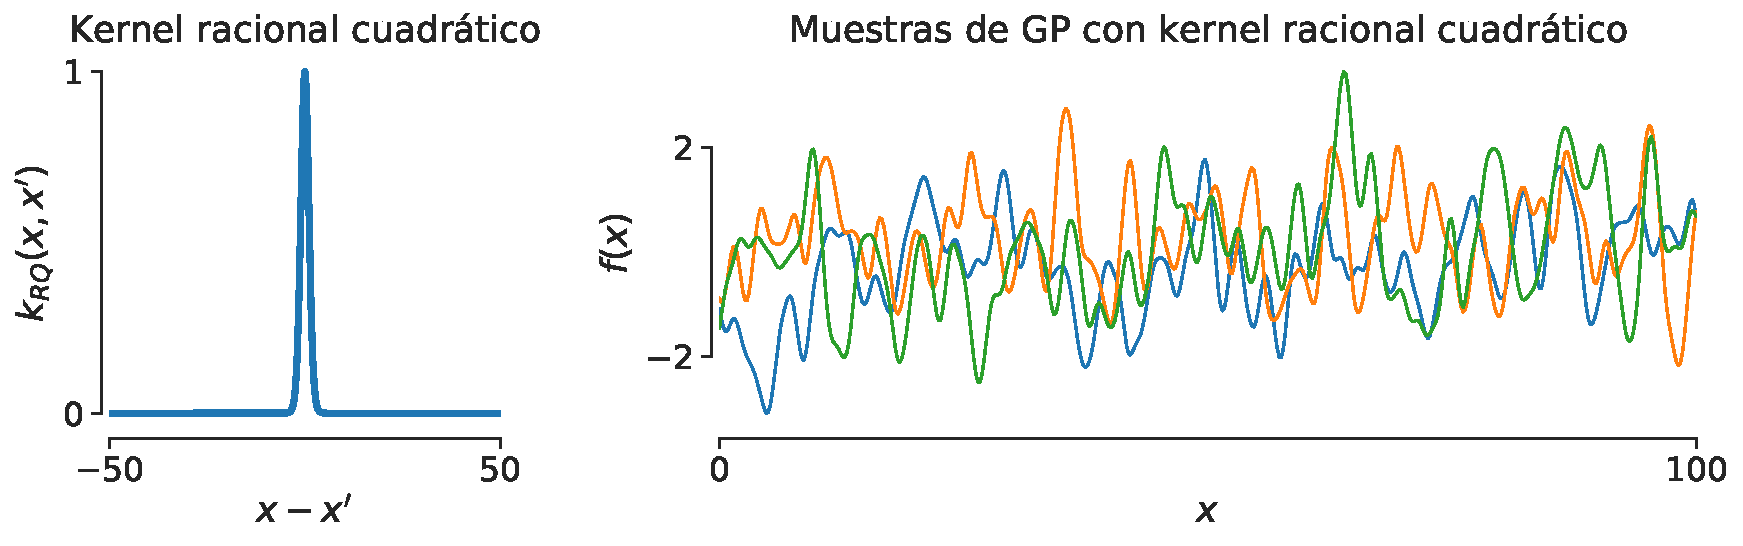
\includegraphics[width=0.9\textwidth]{../img/cap8_muestras_RQ}}
	    \caption{Kernel \textit{Rational Quadratic}, en la izquierda se muestra la covarianza en función de su argumento $\tau=x-x'$, a la derecha de un $\gp$ usando un kernel RQ.}
    \end{figure}

    
\end{frame}

\begin{frame}{Kernel Periódico y localmente periódico}
    
    Descrito por las ecuaciones:

    \begin{equation*}
        K_{P}(x, x') = \sigma^2 \exp\left(-\frac{2\sin^2\left(\pi |x- x'| / p \right)}{\ell^2 } \right)
    \end{equation*}
    
    \begin{equation*}
        K_{LP}(x, x') = \sigma^2  \exp\left(-\frac{\left(x- x' \right)^2}{2\ell^2 } \right) \exp\left(-\frac{2\sin^2\left(\pi |x- x'| / p \right)}{\ell^2 } \right)
    \end{equation*}

    Donde el parámetro $p$ controla el periodo de la función \pause

    \begin{figure}[H]
        \centering
        \visible<2->{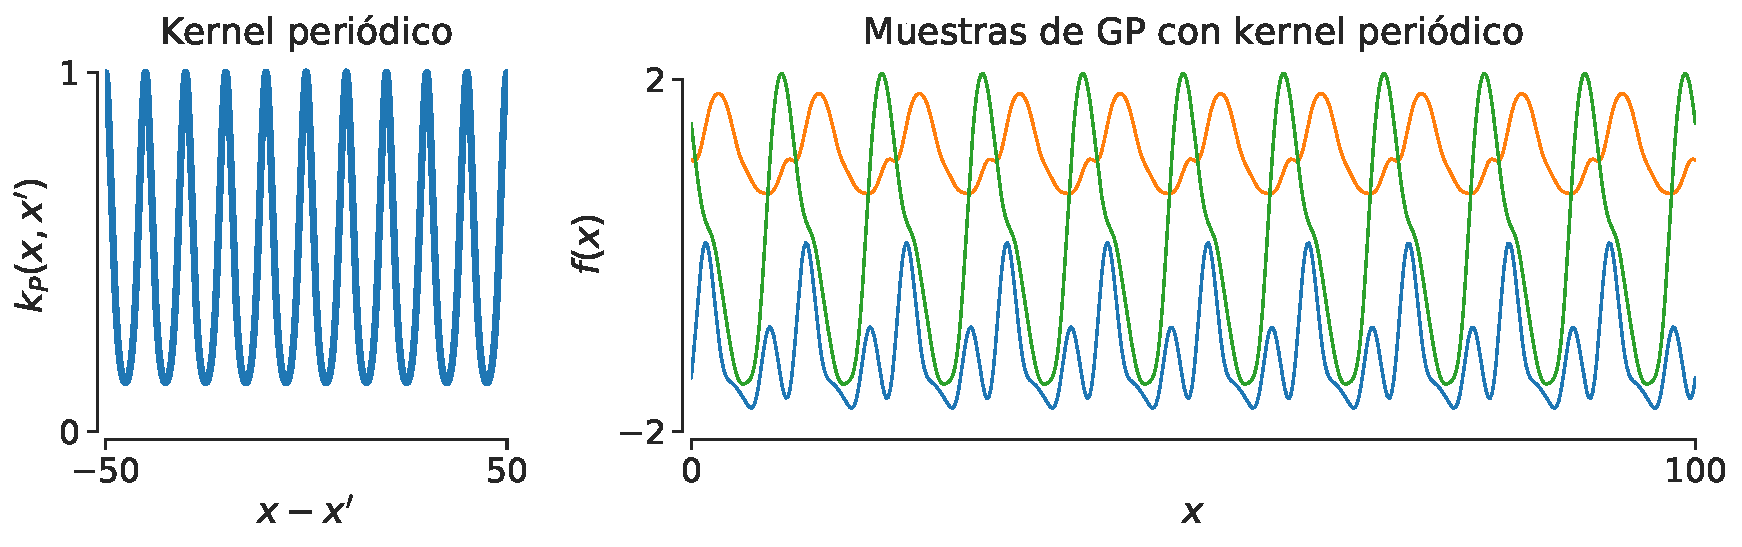
\includegraphics[width=0.9\textwidth]{../img/cap8_muestras_P.pdf}}
        \caption{Kernel periódico, en la izquierda se muestra la covarianza en función de su argumento $\tau=x-x'$, a la derecha de un $\gp$ usando un kernel periódico.}
    \end{figure}
 

    
\end{frame}

\section{Extensiones de un $\gp$}

\begin{frame}{Extensiones de un $\gp$ - Clasificación}
    \begin{wrapfigure}{r}{0.35\textwidth}
        \centering
        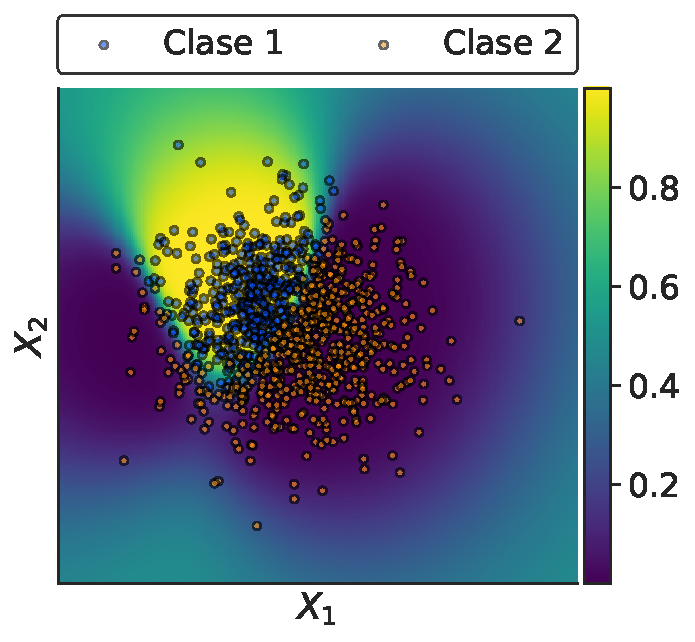
\includegraphics[width=0.3\textwidth]{../img/cap8_classificacion}
        \caption{$\gp$ de clasificación utilizando datos sintéticos. Este clasificador entrega una densidad de probabilidad en vez de una sola función de decisión.}\label{fig:gp_8}
        \end{wrapfigure} 
        
        Hemos visto como usar un $\gp$ para regresión, pero este también puede usado para clasificación, para esto simplemente ``pasamos'' nuestro $\gp$ por una función logística, para así obtener un prior sobre $\sigma\left(f(x)\right)$ donde $\sigma$ es la función logística. Sin embargo esto trae consigo un problema, pues ahora la distribución posterior a las observaciones no se tiene de forma analítica como para el caso de regresión, esto lleva a que tengamos que recurrir a métodos aproximado de inferencia. Una solución simple es utilizar la aproximación de Laplace, pero si se quieren aproximaciones más fidedignas métodos más complejos pueden ser usados como \textit{Expectation Maximization} y métodos MCMC.
    
\end{frame}

\begin{frame}{Extensiones de un $\gp$ - Selección automática de features}
    Un $\gp$ define una densidad de probabilidad sobre funciones, donde estas funciones son del tipo $f: \mathbb{R}^D \rightarrow \mathbb{R}$, con $D$ es finito, este es nuestra dimensión de entrada o ``características''. Haciendo un pequeño cambio en nuestra función kernel podemos hacer que esta automáticamente seleccione las entradas más relevantes con el problema, es decir realice una selección de características automática.
    \vspace{0.2cm} \pause

    Consideremos el siguiente Kernel 
        \begin{equation*}
        k(x, x') = \sigma^2 \exp\left( -\sum_{d=1}^{D} \frac{(x_d - x_d')^2}{2\ell_d^2}\right)
        \end{equation*} \pause 
    
    
    vemos que es una multiplicación de kernels SE, donde se tiene un \textit{lenghtscale} por cada entrada $\ell_d$, sabemos que mientras más grande es este $\ell_d$ menos flexible será el $\gp$ respecto a cambios en ese eje, haciendo que las funciones del proceso dependan cada vez menos de la componente $d$ a medida que $\ell_d \rightarrow \infty$. De esta forma se puede controlar de forma automática la relevancia de cada eje del conjunto de entrada, pues los parámetros del kernel se obtienen en el entrenamiento. De esta forma estamos optimizando también en que grado afecta cada variable en nuestra predicción.

\end{frame}

\begin{frame}{Extensiones de un $\gp$ - Multi output $\gp$}
    Hasta el momento solo hemos hablado de $\gp$ cuando nuestro proceso es solo una dimensión de salida. Se pueden extender los procesos Gaussianos a funciones de más de una salida o canal, donde ahora la función de covarianza $k(x, x')$ no entrega un escalar sino una matriz definida positiva, donde la diagonal corresponde a la covarianza del canal o autocovarianza y los elementos fuera de la diagonal corresponden a las covarianzas cruzadas o cross-covarianza. Este tipo de procesos Gaussianos aumentan considerablemente de complejidad al diseñar funciones de covarianza.

    \vspace{0.2cm} \pause

    Dado un número $m$ de canales, se tendrán $m$ funciones de autocovarianza y ahora $m(m-1)/2$ funciones de covarianza y $k(x, x')$ será una matriz de $m\times m$. El desafio está en diseñar o escoger estas funciones de tal forma que para cualquier par de puntos $x$, $x'$ la matriz $k(x, x')$ sea definida positiva.

    \vspace{0.2cm} \pause

    Una opción simple es asumir que los canales son independientes entre sí, lo que equivale a entrenar independientemente $m$ procesos Gaussianos, uno para cada canal, esto facilita el diseño de las funciones de covarianza pero hace que se pierdan relaciones entre los canales.
 



    
\end{frame}




\begin{frame}
  \titlepage
\end{frame}




%Quitar de comentarios apenas se agregue alguna referencia 
%\bibliography{../capitulos/referencias} %Bibliografía
%\bibliographystyle{apacite}
\end{document} 